\documentclass[a4paper,11pt]{article}
\usepackage[utf8]{inputenc}  % Linux, macOS: enable non-English characters
%\usepackage[latin1]{inputenc}    % Windows: enable non-English characters
\usepackage{fullpage}

%% Colours (used only in macros.tex, and not to be used here):
\newcommand{\blue}[1]{{\color{blue}#1}}
\newcommand{\green}[1]{{\color{green}#1}}
\newcommand{\red}[1]{{\color{red}#1}}

\renewcommand{\thepart}{\arabic{part}}
\renewcommand{\thesection}{\Alph{section}}

%% Useful packages:
\usepackage[boxed]{algorithm}   % drop [boxed] is no box around algorithm wanted
\usepackage[noend]{algorithmic} % drop [noend] if endif, endwhile, etc wanted
\renewcommand{\algorithmiccomment}[1]{\hfill // #1}
\usepackage{alltt}
\usepackage{amsmath}
\usepackage{amssymb}
\usepackage{array}
\usepackage[british]{babel}
\usepackage{booktabs}
\usepackage{cancel}  % provides \cancel
\usepackage[dvipsnames]{xcolor}  % supersedes color
\usepackage{colortbl}  % provides \cellcolor
\usepackage[nocenter]{cwpuzzle}  % provides Sudoku
\usepackage{graphicx}
\usepackage{logicpuzzle}  % provides kakuro
\definecolor{kakuro}{RGB}{155,206,167}
\kakurosetup{color=kakuro}
\usepackage{mathtools} \mathtoolsset{showonlyrefs}  % provides \coloneqq
\usepackage{multicol}
\usepackage{multirow}
\usepackage{pdflscape}  % provides "landscape" environment
\usepackage{pgfplots} \pgfplotsset{compat=1.12}  % was 1.9, but gave errors?!
%\usepackage{rotating}  % provides "sideways[table]" environments
\usepackage{tikz}
\usetikzlibrary{arrows,automata,calc,trees,positioning,decorations.markings}
\usepackage{xspace}
\usepackage{hyperref}
\hypersetup{linkcolor=black}  % should always be last package

%% Fancy characters:
\usepackage{pifont}
%\newcommand{\scissors}{\ding{36}}
%\newcommand{\phone}{\ding{37}}
%\newcommand{\aircraft}{\ding{40}}
%\newcommand{\envelope}{\ding{41}}
\newcommand{\handpoint}{\ding{43}}
%\newcommand{\victory}{\ding{44}}
%\newcommand{\handwrite}{\ding{45}}
\newcommand{\tick}{\ding{51}}
\newcommand{\notick}{\ding{55}}
\DeclareSymbolFont{extraup}{U}{zavm}{m}{n}
%\DeclareMathSymbol{\varclubsuit}{\mathalpha}{extraup}{84}
%\DeclareMathSymbol{\varspadesuit}{\mathalpha}{extraup}{85}
\DeclareMathSymbol{\varheartsuit}{\mathalpha}{extraup}{86}
\DeclareMathSymbol{\vardiamondsuit}{\mathalpha}{extraup}{87}

%% Styles:
\newcommand{\stressed}[1]{\textbf{\textit{#1}}}
\newcommand{\todo}[1]{\green{#1}}  % show to-do items in green
%\newcommand{\todo}[1]{}           % omit to-do items
\newcommand{\done}[1]{\blue{#1}}   % show done  items in blue
%\newcommand{\done}[1]{#1}         % show done  items in black

%% Algorithms:
\newcommand{\EndIf}{\textbf{~end~if}}
\newcommand{\Function}{\textbf{function~}}
\newcommand{\IfThen}[2]{\If#1\Then#2\EndIf}  % use when \IF unsuitable
\newcommand{\In}{\textbf{~in~}}
\newcommand{\Invariant}[1]{{\bf invariant:} #1}
%\newcommand{\IsAssigned}{\gets}
\newcommand{\IsAssigned}{\coloneqq}
\newcommand{\Let}[2]{\textbf{let~}#1\In#2}
\newcommand{\PostCond}[1]{\textbf{post:} #1}
\newcommand{\PreCond}[1]{\textbf{pre:} #1}
\newcommand{\Return}{\textbf{return~}}  % use when \RETURN unsuitable
\newcommand{\Select}{\textbf{pick}}
\newcommand{\Variant}[1]{{\bf variant:} #1}

%% Automata:
\newcommand{\Alphabet}{\Sigma}
\newcommand{\Alternation}[2]{#1|#2}           % of regular expressions
\newcommand{\Concat}[2]{#1 \cdot #2}          % of strings
\newcommand{\DFA}{\mathcal{A}}
\newcommand{\EmptyString}{\epsilon}
\newcommand{\Kleene}[1]{#1^*}                 % of a regular expression
\newcommand{\Language}[1]{\mathcal{L}({#1})}  % of a regular expression
\newcommand{\RegEx}[1]{\mathbf{#1}}           % transforms symbol into reg.ex.

%% CP & Gecode & MiniZinc:
\newcommand{\AnyCond}[1]{\text{Any}(#1)}
\newcommand{\BinPacking}{\Constraint{binpacking}}
\newcommand{\BoundedCond}[1]{\text{Bounded}(#1)}
\newcommand{\Channel}{\Constraint{channel}}
\newcommand{\Circuit}{\Constraint{circuit}}
\newcommand{\CondSet}[1]{\text{PropConds}(#1)}
\newcommand{\Conds}[2]{\text{Conds}(#1,#2)}
%\newcommand{\Constraint}[1]{\textsc{#1}}
\newcommand{\Constraint}[1]{\texttt{#1}}
\newcommand{\Cumulative}{\Constraint{cumulative}}
\newcommand{\DepProps}{\textit{DepProps}}
\newcommand{\DFE}{\text{DFE}}
\newcommand{\Distinct}{\Constraint{distinct}}
\newcommand{\Domain}[1]{\textnormal{dom}(#1)}
\newcommand{\Element}{\Constraint{element}}
\newcommand{\Extensional}{\Constraint{extensional}}
\newcommand{\Failed}{\text{Failed}}
\newcommand{\FailedCond}[1]{\text{Failed}(#1)}
\newcommand{\FixedCond}[1]{\text{Fixed}(#1)}
\newcommand{\Fixpoint}{\text{AtFixpt}}
\newcommand{\GlobalCardinality}{\Constraint{count}}
\newcommand{\Linear}{\Constraint{linear}}
\newcommand{\MaxCond}[1]{\text{Max}(#1)}
\newcommand{\MinCond}[1]{\text{Min}(#1)}
\newcommand{\ModVars}{\textit{ModVars}}
\newcommand{\NoneCond}[1]{\text{None}(#1)}
\newcommand{\NValues}{\Constraint{nvalues}}
\newcommand{\Path}{\Constraint{path}}
\newcommand{\Precede}{\Constraint{precede}}
\newcommand{\Propagate}{\text{Propagate}}
%\newcommand{\Reifies}[2]{#1\Leftrightarrow#2}
\newcommand{\Reifies}[2]{#2\Leftrightarrow#1}  % layout as in MiniZinc
\newcommand{\Subsumed}{\text{Subsumed}}
\newcommand{\Unary}{\Constraint{unary}}
\newcommand{\Unknown}{\text{Unknown}}
\newcommand{\Variables}[1]{\text{var}(#1)}

%% Mathematics:
\newcommand{\AbsValue}[1]{\left\lvert#1\right\rvert}
\newcommand{\Cardinality}[1]{\left\lvert#1\right\rvert}
%\newcommand{\Cardinality}[1]{\##1}
\newcommand{\Ceiling}[1]{\left\lceil#1\right\rceil}
\newcommand{\Else}{\textbf{~else~}}
\newcommand{\EmptySet}{\varnothing}
\newcommand{\Floor}[1]{\left\lfloor#1\right\rfloor}
\newcommand{\GeqLex}{\geq_\Lex}
\newcommand{\If}{\textbf{if~}}
\newcommand{\Iff}{\Leftrightarrow}
\newcommand{\IfThenElse}[3]{\If#1\Then#2\Else#3}
\newcommand{\Implies}{\Rightarrow}
\newcommand{\Int}{\mathbb{Z}}
\newcommand{\Inter}{\cap}
\newcommand{\Iverson}[1]{\red{\left[{\color{black}#1}\right]}}
\newcommand{\LeqLex}{\leq_\Lex}
\newcommand{\Lex}{\textnormal{lex}}
\newcommand{\LtLex}{<_\Lex}
\newcommand{\Nat}{\mathbb{N}}
\newcommand{\Oh}[1]{\mathcal{O}(#1)}
\newcommand{\Sequence}[1]{\left[#1\right]}
\newcommand{\Set}[1]{\left\{#1\right\}}
\newcommand{\SetComp}[2]{\Set{#1\SuchThat#2}}
\newcommand{\SuchThat}{\mid}
\newcommand{\Then}{\textbf{~then~}}
\newcommand{\Tuple}[1]{\left\langle#1\right\rangle}
\newcommand{\Union}{\cup}

%% Tools:
\newcommand{\Gecode}{Gecode\xspace}
\newcommand{\GIST}{GIST\xspace}
\newcommand{\MiniModel}{Mini\-Model\xspace}
\newcommand{\MiniZinc}{Mini\-Zinc\xspace}
\newcommand{\Python}{Python\xspace}

\usepackage{listings}
\usepackage{courier} % \texttt{...} gives thinner text and /\ displays OK

\newcommand\mznfont{\fontfamily{pcr}\selectfont}

\lstdefinelanguage{Mzn}
{
  morekeywords={
  %
  array, par, var, opt, constraint, solve, satisfy, minimize,
  maximize, output, include, let, in, set, of, if, then, else, endif,
  ann, annotation, bool, enum, float, int, string, where, function,
  predicate, true, false, not, assert, trace,
  % ???:
  any, list, op, record, test, tuple, type
  %
  },
  %
  keywords=[2]{
  %
  forall, sliding_sum, symmetry_breaking_constraint,
  implied_constraint, redundant_constraint, all_different,
  alldifferent, alldifferent_except_0, alldiff, element, circuit,
  subcircuit, card, bool2int, inter, count, regular, table, xor,
  exists, xorall, iffall, clause, intersect, diff, symdiff, subset,
  superset, concat, join, length, int_lt_reif, int_lin_eq_reif,
  bool_imply, array_bool_or, all_different_int, int_ne, at_least,
  at_most, exactly, count_eq, count_leq, count_geq, count_gt, nvalue,
  bin_packing, bin_packing_capa, bin_packing_load, diffn,
  global_cardinality, global_cardinality_closed,
  global_cardinality_low_up, global_cardinality_low_up_closed,
  inverse, cumulative, disjunctive, decreasing, increasing, sort,
  arg_sort, value_precede, value_precede_chain, lex_less, lex_lesseq,
  lex_greater, lex_greatereq, lex2, int_lin_eq, bool_lin_eq, knapsack,
  partition_set, member, reverse,
  % from ???:
  abort, abs, acosh, array_intersect, array_union, array1d, array2d,
  array3d, array4d, array5d, array6d, asin, atan, bool2int, card,
  ceil, concat, cos, cosh, dom, dom_array, dom_size, fix, exp, floor,
  index_set, index_set_1of2, index_set_2of2, index_set_1of3,
  index_set_2of3, index_set_3of3, index_set_6of6, int2float, is_fixed,
  join, lb, lb_array, length, ln, log, log2, log10, min, max, pow,
  product, round, set2array, show, show_int, show_float, sin, sinh,
  sqrt, sum, tan, tanh, trace, ub, ub_array, xor, in, subset,
  superset, union, diff, symdiff, intersect, div, mod,
  % annotations:
  is_defined_var, output_var, var_is_introduced, defines_var,
  promise_total, bounds, domain, bool_search, int_search, seq_search,
  set_search, input_order, first_fail, anti_first_fail, smallest,
  largest, occurrence, most_constrained, max_regret, indomain_min,
  indomain_max, indomain_middle, indomain_median, indomain,
  indomain_random, indomain_split, indomain_reverse_split,
  indomain_interval, outdomain_max, outdomain_median, outdomain_min,
  outdomain_random, complete
  % 
  },
  sensitive=true,
  basicstyle=\mznfont,
  commentstyle=\color[rgb]{0.9,0.1,0.1},
  keywordstyle=\color[rgb]{0,0.5,0},
  keywordstyle=[2]\color{blue},
  stringstyle=\color{orange},
  tabsize=2,
  frame=none,
  % identifierstyle = \it,
  numbers=left,
  stepnumber=1,
  numberstyle=\tiny,
  numbersep=5pt,
  xleftmargin=0pt, % numbers will be in the margins!
  columns=fixed, % same width for all characters
  % columns=flexible,
  % columns=fullflexible,
  morecomment=[l]{\%},
  morestring=[b]",
  % morestring=[d]',
  showstringspaces=false,
  mathescape=true,
  breaklines=true,
  % prebreak=\raisebox{0ex}[0ex][0ex]{\ensuremath{\space\red{\swarrow}}},%\hookrightarrow
  %postbreak=\raisebox{0ex}[0ex][0ex]{\ensuremath{\hookrightarrow\space}},%\hookrightarrow
  breakatwhitespace=true,
  breakindent=10pt, % was: 20pt
  moredelim=**[is][\color{Melon}]{@}{@},
  escapeinside={{<@}{@>}}
}
%% Write "\begin{frame}[fragile]" for a slide using either of the
%% following two listing environments, which have unnumbered
%% respectively numbered lines:
\lstnewenvironment{mzn}[1][]{\lstset{language=Mzn,#1}}{}
\lstnewenvironment{mznno}[1][]{\lstset{language=Mzn,numbers=none,xleftmargin=0pt,#1}}{}
%% Inline a code snippet, without respectively with the comprehension bar (|):
\newcommand{\mzninline}[1]{\lstinline[{language=Mzn}]|#1|}
\newcommand{\mzninlinebar}[1]{\lstinline[{language=Mzn}]!#1!}


\title{\textbf{Modelling and Problem Solving (CS4530) \\
    TU Delft -- YEAR \\  % Replace by which academic year this is
    Report for Assignment~$1$ \\
    Group number $NN$  % Replace by your group number
  }
}

%% Replace by your name(s)
\author{Clara CLÄVER \and Whiz KIDD}

\date{\today}

\begin{document}

\maketitle

%% Delete this paragraph:
\noindent
This document shows the ingredients of a good assignment or project
report for this (part of the) course.  It is thanks to Pierre Flener, Uppsala University.
%
This document's \LaTeX\ source code also exemplifies almost everything you need to
know about \LaTeX\ in order to typeset a professional-looking
assignment or project report (for this course).
%
Use the source code of this document as a starting point for
imitation, whether you use \LaTeX\ or not, and delete everything
irrelevant.  The \LaTeX\ source code of this document also contains
useful comments.  The usage of \LaTeX\ is \stressed{optional}, but
highly recommended, for reasons that will soon become clear to those
who have never used it before.  Any learning time of \LaTeX\ is
\stressed{outside} the time budget of this course, but will hugely pay
off, if not in this course then in the next course(s) you take and
when writing a thesis or other scientific report.
%
\bigskip

%% Delete this paragraph:
Address \stressed{each} task of \stressed{each} problem, using the
numbering and ordering in which the problems and tasks appear in the
assignment statement:
\begin{itemize}
\item For each task requiring a model, follow the advice and structure
  of Section~\ref{sec:minMagicSquare:model}.
\item For each task requiring an evaluation, follow the structure of
  Section~\ref{sec:minMagicSquare:eval}.
\end{itemize}
Delete all unnecessary text and suitably replace all other text in
this document.

%% Put a suitable heading here:
\part{The Minimal Magic Square Problem}
\setcounter{section}{0} % reset the section counter for each part

% Note the non-breaking spaces, typeset via ~, between numbers and
% their units:
All experiments were run under
% specs of the ThinLinc machines of the IT department:
Linux Ubuntu~18.04 ($64$~bit) on an Intel Xeon E5520 of $2.27$~GHz,
with $4$~processors of $4$~cores each, with a $70$~GB RAM and an
$8$~MB L3 cache.%
%
%% Delete this footnote:
\footnote{Hint: Under Linux, do \texttt{lscpu} to find this
  information.  Under macOS, you find this information via ``About
  This Mac'' in the Apple menu.}
%
%% Delete or replace this sentence:
(If different hardware was used for different tasks, then justify this
and replicate a paragraph like this one within each relevant section.)

%% Put a suitable heading here:
\section{Heading for Task~A}

(Write your answer for Task~A here.)

%% Put a suitable heading here:
\section{Use Appropriate Headings for the Sections}

%% Replace this sentence by something suitable:
(Remember that this document is a guideline, so that you should change
its structure and text when appropriate.)

\section{Model}
\label{sec:minMagicSquare:model}

% You need NOT describe a problem that is fully described in the
% assignment statement!

%% Delete this entire paragraph, but follow its instructions:
A CP model (e.g., \MiniZinc~\cite{MiniZinc}) \stressed{must} include comments
that explain:
\begin{itemize}
\item the parameters that are not part of the possibly provided
  skeleton code;
\item the decision variables, and which problem constraints, if any,
  they automatically enforce;
\item the redundant decision variables; if none, then justify this in
  Section~\ref{sec:minMagicSquare:desc};
\item the problem constraints not enforced by the choice of decision
  variables;
\item the objective, including possibly the objective function;
\item the channelling constraints; if none, then justify this in
  Section~\ref{sec:minMagicSquare:desc};
\item the implied constraints; if none, then justify this in
  Section~\ref{sec:minMagicSquare:desc};
\item the symmetry-breaking constraints; if none, then justify this in
  Section~\ref{sec:minMagicSquare:desc};
\item the (CP/LCG) inference annotations; if none, then justify this in
  Section~\ref{sec:minMagicSquare:desc};
\item the (CP/LCG) search annotation; if none, then justify this in
  Section~\ref{sec:minMagicSquare:desc}.
\end{itemize}
\stressed{The quality of model comments is considered while grading.}
%
See Listing~\ref{model:minMagicSquare} for an example of sufficiently
good model comments.
%
You \stressed{must} include your model in your report in addition to
uploading it as a separate file (so that we can run it).

\lstinputlisting[language=Mzn,caption={A \MiniZinc model for the
  Minimal Magic Square
  problem},label=model:minMagicSquare]{minMagicSquare.mzn}

\subsection{Description}
\label{sec:minMagicSquare:desc}

%% Delete this paragraph, but follow its instructions:
(Provide, here in the report, a more detailed explanation
(\emph{i})~why each redundant decision variable is deemed useful,
(\emph{ii})~why each channelling, implied, and symmetry-breaking
constraint is correct, as well as (\emph{iii})~how the inference and
search annotations were chosen.  Use any combination of in-lined code,
mathematical notation, and plain English to explain your choices.)

\paragraph{Redundant Decision Variables and Channelling Constraints.}
We do not think that redundant decision variables could be usefully
introduced into our model, which thus also has no channelling
constraints.

\paragraph{Implied Constraints.}
Since the sum of each row must be equal to the magic sum, and since
all values from $1$ to $\mzninline{n}^2$ must occur exactly once in
the magic square, it is implied that the sum of the rows is the sum of
the entire magic square, that is \mzninline{n * magicSum =
  sum(1..n*n)}.  Since \mzninline{n} is a parameter, this implied
constraint actually fixes the decision variable \mzninline{magicSum},
namely to \mzninline{sum(1..n*n) div n} (that is to
\mzninline{(n*n*n+n) div 2}), hence:
%
\lstinputlisting[language=Mzn,firstnumber=25,firstline=25,lastline=25]{minMagicSquare.mzn}
%
We reckon this constraint is useful to solvers of all technologies and
hence we do \emph{not} flag it using the
\mzninline{implied_constraint} special predicate.

\paragraph{Symmetry-Breaking Constraints.}
A magic square has rotation and reflection symmetries.
%
The rotation symmetries for $90$, $180$, and $270$ degrees and the
reflection symmetries for the horizontal axis, vertical axis, and
up-right diagonal can be broken by requiring the top-left corner of
the magic square to be smaller than the other corners:
% 
\lstinputlisting[language=Mzn,firstnumber=30,firstline=30,lastline=34]{minMagicSquare.mzn}
%
The reflection symmetry for the down-right diagonal can be broken by
requiring the bottom-left corner to be smaller than the top-right
corner:
% 
\lstinputlisting[language=Mzn,firstnumber=37,firstline=37,lastline=37]{minMagicSquare.mzn}
%
As recommended, these constraints are flagged using the
\mzninline{symmetry_breaking_constraint} special predicate.

\paragraph{Inference Annotations.}
We leave the sensible choice of inference for the linear equality
constraints (lines~14--19) and the linear objective function (line~48)
to each CP and LCG backend, assuming it is domain consistency for
smaller values of \mzninline{n} and bounds consistency for larger
values, the threshold being probably backend-specific.

The implied linear equality constraint (line~25) has only one decision
variable and functionally determines it, hence this constraint will be
immediately satisfied and needs no annotation.

All the symmetry-breaking constraints (lines~30--37) are inequalities
on two decision variables, where we assume domain consistency under
\emph{each} CP and LCG backend, as this is as cheap to achieve as the
weaker bounds consistency.

This leaves the all-difference constraint (line~11), for which we
explicitly suggest domain consistency.

\paragraph{Search Annotation.}
Since the four corners of the magic square correspond to the only
decision variables of the objective function and furthermore occur in
more constraints than the other cells of the magic square, namely
additionally in the diagonal and symmetry-breaking constraints, we
suggest a sequence of two search phases.
%
First, we search on the four corners.  We use the variable selection
strategy \mzninline{input_order} as the order of those four decision
variables does not matter.  We use the value selection strategy
\mzninline{indomain_split} in order to bisect the domain of the chosen
decision variable, because bisection is known to be good in the
presence of arithmetic constraints (only the all-difference constraint
in line~11 is not arithmetic), starting on the lower half, because the
objective function is to be minimised.
%
Second, we search on the remaining variables.  We use the strategy
\mzninline{occurrence} to select a decision variable occurring in the
largest number of constraints, as the non-corners of the diagonals are
more constrained than the other remaining cells.  We use the value
selection strategy \mzninline{indomain_split} for the same reason as
in the first phase.

\subsection{Implementation}
\label{sec:minMagicSquare:impl}

The described model, with the prescribed comments, is uploaded as file
\texttt{minMagicSquare.mzn}.

\paragraph{Compilation and Running Instructions.}
%% This will help the teachers grade your model:
To compile and run \texttt{minMagicSquare.mzn} one must supply a value
for the parameter \texttt{n} using the \texttt{-D} option in the
command line.
%
Assuming that \texttt{mzn-backend} is one of the backends provided for
the course, the model can be compiled and run for \texttt{n=5} by
typing \texttt{mzn-backend minMagicSquare.mzn -D "n=5"} at the command
line.

\paragraph{Sample Test-Run Command.}
\begin{verbatim}
> mzn-gecode minMagicSquare.mzn -D "n=5"
[...snip...]
----------
Magic sum: 65
Magic square: 
3 14 17 24 7
23 8 5 9 20
22 4 25 1 13
11 18 2 19 15
6 21 16 12 10
CornerSum: 26
Corners: [3, 7, 6, 10]
----------
==========
Finished in 1m 8s
\end{verbatim}

\section{Evaluation}
\label{sec:minMagicSquare:eval}

\newcommand{\TimeOut}{600}  %% in CPU seconds: Choose a suitable value!

%% Delete this first sentence:
(Choose, without justification, any solver backends you want, as long as you
cover all the relevant technologies.)
%
We have chosen the backends for Gecode, Chuffed, Gurobi, OscaR.cbls,
and Lingeling.

%% Delete this paragraph, but follow its instructions:
(Give a table of experiment results for the chosen backends, and
analyse it.  Provide an ideally experimental justification for the
redundant decision variables, channelling constraints, implied
constraints, symmetry-breaking constraints, inference annotations, and
search annotation.)

\paragraph{Experiments.}
Table~\ref{tab:res:minMagicSquare} gives the results for various
values of~\mzninline{n} on our Minimal Magic Square model.
%
The time-out was $\TimeOut$~seconds.

\begin{landscape}
  \begin{table}[t]  %% Float the table towards the top [t] of its page
    \centering
    \begin{tabular}{rrrrrrrrrrr}  %% right [r] for decimal-point alignment
%     \toprule
      Technology
      & \multicolumn{2}{c}{CP}
      & \multicolumn{2}{c}{LCG}
      & \multicolumn{2}{c}{MIP}
      & \multicolumn{2}{c}{CBLS}
      & \multicolumn{2}{c}{SAT} \\
      \cmidrule(lr){02-03} \cmidrule(lr){04-05} \cmidrule(lr){06-07}
      \cmidrule(lr){08-09} \cmidrule(lr){10-11}
      Solver  %% Make your own pick of backends for each technology!
      & \multicolumn{2}{c}{Gecode}
      & \multicolumn{2}{c}{Chuffed}
      & \multicolumn{2}{c}{Gurobi}
      & \multicolumn{2}{c}{OscaR.cbls}
      & \multicolumn{2}{c}{Lingeling} \\
      \cmidrule(lr){02-03} \cmidrule(lr){04-05} \cmidrule(lr){06-07}
      \cmidrule(lr){08-09} \cmidrule(lr){10-11}
      Backend
& \multicolumn{2}{c}{mzn-gecode}
& \multicolumn{2}{c}{mzn-chuffed}
& \multicolumn{2}{c}{mzn-gurobi}
& \multicolumn{2}{c}{mzn-oscar-cbls}
& \multicolumn{2}{c}{mzn-picat} \\
\cmidrule(lr){02-03} \cmidrule(lr){04-05} \cmidrule(lr){06-07}
\cmidrule(lr){08-09} \cmidrule(lr){10-11}
\texttt{n}
& \texttt{CornerSum} & time
& \texttt{CornerSum} & time
& \texttt{CornerSum} & time
& \texttt{CornerSum} & time
& \texttt{CornerSum} & time \\
\midrule
3 & 20 & 0.422 & 20 & 0.954 & 20 & 1.268 & 20 & t/o & 20 & 1.262 \\
4 & 34 & 0.372 & 34 & 0.680 & 34 & 1.210 & 34 & t/o & 34 & 8.297 \\
5 & 26 & 68.100 & 26 & t/o & 26 & 46.645 & 36 & t/o & 27 & t/o \\
6 & -- & t/o & -- & t/o & 26 & 65.681 & -- & t/o & 39 & t/o \\

%     \bottomrule
    \end{tabular}
    %% Adapt this caption to your problem:
    \caption{Results for our Minimal Magic Square model.
      %
      In the `time' column, if the reported time is less than the
      time-out (\TimeOut~seconds here), then the reported objective
      value in the `\texttt{CornerSum}' column was \emph{proven}
      optimal;
      % 
      else the time-out is indicated by `t/o' and the reported
      objective value is either the best value found, but \emph{not}
      proven optimal, before timing out,
      % 
      or~`--', indicating that no feasible solution was found before
      timing out.
      % 
      If the reported time is~`--', then that instance was not
      run on that backend, as the latter timed out on a smaller instance
      (this is normally not a correct assumption, as larger instances
      can be easier, but for the assignments of this course this
      assumption is fine).}
    \label{tab:res:minMagicSquare}
  \end{table}
\end{landscape}

\paragraph{Analysis.}
%% Delete this first sentence:
(Refer to and explain the table(s), draw some conclusions from the
experiment, and analyse:)
%
We observe that the chosen MIP backend wins overall, as it is the only
one not to time out for the largest chosen instance, with
$\mzninline{n}=6$.
% 
The chosen MIP and SAT backends scale best, as they are the only ones
to establish feasibility for $\mzninline{n}=6$, even though the SAT
objective value of~$39$ at time-out is far above the minimum of~$26$
proven by the MIP backend.
%
On small instances, with $\mzninline{n} \in \Set{3,4}$, the chosen CP
backend wins, narrowly defeating the chosen LCG backend followed by
the MIP and SAT backends.  The SAT backend is the only one where
$\mzninline{n}=4$ is harder than the smaller $\mzninline{n}=3$.
%
Starting from the medium instance, with $\mzninline{n}=5$, the MIP
backend clearly wins, with only the CP backend also not timing out,
the LCG backend finding but not proving the minimum, and the SAT
backend missing the minimum by one unit.
%
The chosen CBLS backend always times out, because local search can by
construction not prove minima on problems, such as here, where the
trivial lower bound (namely $10 = 1 + 2 + 3 + 4$ here) on the
objective value is not feasible; it finds the known minima for
$\mzninline{n} \in \Set{3,4}$, but is far above the known minimum for
$\mzninline{n}=5$ and cannot establish feasibility for
$\mzninline{n}=6$ before timing out.

\paragraph{Redundant Decision Variables and Channelling Constraints.}
Our model was argued in Section~\ref{sec:minMagicSquare:desc} not to
benefit from any redundant decision variables and their channelling
constraints, hence there is no runtime impact analysis to make.

\paragraph{Implied Constraints.}
The huge runtime impact of our unique implied constraint (line~25),
fixing the decision variable occurring in all constraints, is not
experimentally demonstrated here, because our experiments (not shown
here for time reasons) confirmed our hunch that it is absolutely
crucial, for all solving technologies and all solvers.

\paragraph{Symmetry-Breaking Constraints.}
The huge runtime impact of our symmetry-breaking constraints is as
follows, illustrated here only for the CP solver Gecode, which ought
to be representative for backends enabling the symmetry-breaking
constraints: in the presence of the search annotation (evaluated
separately below), the most difficult instance that does not time out
(namely $\mzninline{n}=5$) is solved in $68$~seconds with the
symmetry-breaking constraints, but takes $377$~seconds without those
constraints.

\paragraph{Inference Annotations.}
The huge runtime impact of our unique inference annotation (in
line~11) is not experimentally demonstrated here, because our
experiments (not shown here for time reasons) revealed that it is
absolutely crucial for CP and LCG solvers (and because we do not know
the backend defaults).

\paragraph{Search Annotation.}
The huge runtime impact of our search annotation is as follows,
illustrated here only for the CP solver Gecode, which ought to be
representative for CP and LCG solvers: in the presence of the
symmetry-breaking constraints (evaluated separately above), the most
difficult instance that does not time out (namely $\mzninline{n}=5$)
is solved in $68$~seconds with the search annotation, but takes
$408$~seconds without that annotation (there is a time-out upon no
symmetry-breaking constraints and no search annotation).

%% Delete this hint:
\paragraph{Hint.}
Use a script, such as the one explained in
\url{http://user.it.uu.se/~gusbj192/courses/M4CO/cheatsheet.pdf} and available on Brightspace, that
conducts the final experiments for you and directly generates a result
table (see the \LaTeX\ source code of
Table~\ref{tab:res:minMagicSquare}) that is automatically imported
(rather than manually copied) into your report: each time you change
the model, it suffices to re-run that script and re-compile your
report, in your absence, without any tedious number copying!

\section*{Feedback to the Teaching Staff}

%% Fill in:
(Please write a paragraph, which will not be graded, describing your
experience with this assignment: which aspects were too difficult or
too easy, and which aspects were interesting or boring?  This may help
us improve the course for the next year.)

\section*{Crash Report}

%% Fill in:
(For instances where no result is reported, due to a solver crashing
or the \MiniZinc toolchain failing to compile the model, please
include an error message, if there is any.  For example:)

\paragraph{largecumulative.mzn} For the larger instances,
mzn-oscar-cbls crashes with the following exception, which seems to be
caused by the JVM not being allocated enough heap space.

{\tiny
\begin{verbatim}
>./fzn-oscar-cbls -s -t 600 /tmp/tmp.fzn
Exception in thread "main" java.lang.OutOfMemoryError: Java heap space
  at scala.collection.mutable.FlatHashTable$class.growTable(FlatHashTable.scala:217)
  at scala.collection.mutable.FlatHashTable$class.addEntry(FlatHashTable.scala:159)
  at scala.collection.mutable.HashSet.addEntry(HashSet.scala:40)
  at scala.collection.mutable.FlatHashTable$class.addElem(FlatHashTable.scala:139)
  at scala.collection.mutable.HashSet.addElem(HashSet.scala:40)
  at scala.collection.mutable.HashSet.$plus$eq(HashSet.scala:59)
  at oscar.cp.scheduling.constraints.EnergeticReasoning$$anonfun$computeIntervals$1$$anonfun$apply$mcVI$sp$2.apply(EnergeticReasoning.scala:127)
  at oscar.cp.scheduling.constraints.EnergeticReasoning$$anonfun$computeIntervals$1$$anonfun$apply$mcVI$sp$2.apply(EnergeticReasoning.scala:126)
  at scala.collection.TraversableLike$WithFilter$$anonfun$foreach$1.apply(TraversableLike.scala:778)
  at scala.collection.mutable.HashSet.foreach(HashSet.scala:78)
  at scala.collection.TraversableLike$WithFilter.foreach(TraversableLike.scala:777)
  at oscar.cp.scheduling.constraints.EnergeticReasoning$$anonfun$computeIntervals$1.apply$mcVI$sp(EnergeticReasoning.scala:126)
  at oscar.cp.scheduling.constraints.EnergeticReasoning$$anonfun$computeIntervals$1.apply(EnergeticReasoning.scala:126)
  at oscar.cp.scheduling.constraints.EnergeticReasoning$$anonfun$computeIntervals$1.apply(EnergeticReasoning.scala:126)
  at scala.collection.mutable.HashSet.foreach(HashSet.scala:78)
  at oscar.cp.scheduling.constraints.EnergeticReasoning.computeIntervals(EnergeticReasoning.scala:126)
  at oscar.cp.scheduling.constraints.EnergeticReasoning.propagate(EnergeticReasoning.scala:77)
\end{verbatim}
}

% \section*{References}
%
\bibliographystyle{plain}
\bibliography{skeleton}

%% Comment away the following line before submitting:
\newpage
\section*{Checklist before Submitting}

In order to protect yourself against an unnecessary loss of points,
use the following checklist before submitting:
\begin{itemize}
\item Crosscheck your report against the assignment instructions.
\item {\color{red}Remember that when submitting you implicitly certify
    (a)~that your report and all its uploaded attachments were
    produced solely by your team, except where explicitly stated
    otherwise and clearly referenced, (b)~that each teammate can
    individually explain any part starting from the moment of
    submitting your report, and (c)~that your report and attachments
    are not freely accessible on a public repository.}
\item Crosscheck against the technical writing and \LaTeX\ advice
  below.  The \emph{English Style Guide} of Uppsala University at
  \url{https://mp.uu.se/en/web/info/stod/kommunikation-riktlinjer/sprak/eng-skrivregler}
  and the technical-writing \emph{Checklist \& Style Manual} of
  Uppsala's Optimisation group at
  \url{http://optimisation.research.it.uu.se/checkList.pdf} offer many
  further pieces of advice.  Common errors in English usage are
  discussed at \url{https://brians.wsu.edu/common-errors}.
\item Spellcheck all documents, including the comments in the source
  code.
\item Proofread, if not grammar-check, your report at least once per
  teammate.
\item Pay attention to all submission and other instructions in the assignment description, including but not limited to the use of `language-generative' AI tools.  
\end{itemize}

\section*{More \LaTeX\ and Technical Writing Advice\protect\footnote{Thanks to Pierre Flener.}}

Unnumbered itemisation (only to be used when the order of the items
does \emph{not} matter):\footnote{Use footnotes very sparingly, and
  note that footnote pointers are \emph{never} preceded by a space and
  always glued immediately \emph{behind} the punctuation, if there is
  any.}
\begin{itemize}
\item Unnumbered displayed formula:
  \[
  E = m \cdot c^2
  \]
\item Numbered displayed formula, which is cross-referenced somewhere:
  \begin{equation}
    \label{eq:emc2}
    E = m \cdot c^2
  \end{equation}
\item Formula --- the same as formula~(\ref{eq:emc2}) --- spanning
  more than one line:
  \begin{gather*}
    E \\ = m \cdot c^2
  \end{gather*}
\end{itemize}
Numbered itemisation (only to be used when the order of the items
\emph{does} matter):
\begin{enumerate}
\item First do this.
\item\label{item:that} Then do that.
\item If we are not finished, then go back to Step~\ref{item:that},
  else stop.
\end{enumerate}

Tables and elementary mathematics are typeset as exemplified in
Table~\ref{tab:maths}; see
\url{ftp://ftp.ams.org/pub/tex/doc/amsmath/short-math-guide.pdf} for
many more details.

\begin{table}[t] % make it float to the top of a page
  \centering
  \begin{tabular}{rlc} % right left centre
    \toprule
    Topic & \LaTeX\ code & Appearance \\
    \midrule
    Greek letter & \verb|$\Theta,\Omega,\epsilon$| & $\Theta,\Omega,\epsilon$ \\
    multiplication & \verb|$m \cdot n$| & $m \cdot n$ \\
    division & \verb|$\frac{m}{n}, m \div n$| & $\frac{m}{n}, m \div n$ \\
    rounding down & \verb|$\left\lfloor n \right\rfloor$| & $\left\lfloor n \right\rfloor$ \\
    rounding up & \verb|$\left\lceil n \right\rceil$| & $\left\lceil n \right\rceil$ \\
    binary modulus & \verb|$m \bmod n$| & $m \bmod n$ \\
    unary modulus & \verb|$m \equiv n \mod \ell$| & $m \equiv n \mod \ell$ \\
    root & \verb|$\sqrt{n},\sqrt[3]{n}$| & $\sqrt{n},\sqrt[3]{n}$ \\
    exponentiation, superscript & \verb|$n^{i}$| & $n^{i}$ \\
    subscript & \verb|$n_{i}$| & $n_{i}$ \\
    overline & \verb|$\overline{n}$| & $\overline{n}$ \\
    base $2$ logarithm & \verb|$\lg n$| & $\lg n$ \\
    base $b$ logarithm & \verb|$\log_b n$| & $\log_b n$ \\
    binomial & \verb|$\binom{n}{k}$| & $\binom{n}{k}$ \\
    sum & \verb|\[\sum_{i=1}^n i\]| & $\displaystyle\sum_{i=1}^n i$ \\
    numeric comparison & \verb|$\leq,<,=,\neq,>,\geq$| & $\leq,<,=,\neq,>,\geq$ \\
    non-numeric comparison & \verb|$\prec,\nprec,\preceq,\succeq$| & $\prec,\nprec,\preceq,\succeq$ \\
    extremum & \verb|$\min,\max,+\infty,\bot,\top$| & $\min,\max,+\infty,\bot,\top$ \\
    function & \verb|$f\colon A\to B,\circ,\mapsto$| & $f\colon A\to B,\circ,\mapsto$ \\
    sequence, tuple & \verb|$\langle a,b,c \rangle$| & $\langle a,b,c \rangle$ \\
    set & \verb|$\{a,b,c\},\emptyset,\mathbb{N}$| & $\{a,b,c\},\emptyset,\mathbb{N}$ \\
    set membership & \verb|$\in,\not\in$| & $\in,\not\in$ \\
    set comprehension & \verb|$\{i \mid 1 \leq i \leq n\}$| & $\{i \mid 1 \leq i \leq n\}$ \\
    set operation & \verb|$\cup,\cap,\setminus,\times$| & $\cup,\cap,\setminus,\times$ \\
    set comparison & \verb|$\subset,\subseteq,\not\supset$| & $\subset,\subseteq,\not\supset$ \\
    logic quantifier & \verb|$\forall,\exists,\nexists$| & $\forall,\exists,\nexists$ \\
    logic connective & \verb|$\land,\lor,\neg,\Rightarrow$| & $\land,\lor,\neg,\Rightarrow$ \\
    logic & \verb|$\models,\equiv,\vdash$| & $\models,\equiv,\vdash$ \\
    miscellaneous & \verb|$\&,\#,\approx,\sim,\ell$| & $\&,\#,\approx,\sim,\ell$ \\
    dots & \verb|$\ldots,\cdots,\vdots,\ddots$| & $\ldots,\cdots,\vdots,\ddots$ \\
    dots (context-sensitive) & \verb|$1,\dots,n; 1+\dots+n$| & $1,\dots,n; 1+\dots+n$ \\
    parentheses (autosizing) & \verb|$\left(m^{n^k}\right),(m^{n^k})$| & $\left(m^{n^k}\right),(m^{n^k})$ \\
    identifier of $>1$ character & \verb|$\mathit{identifier}$| & $\textit{identifier}$ \\
    hyphen, \emph{n}-dash, \emph{m}-dash, minus & \verb|-|, \verb|--|, \verb|---|, \verb|$-$| & -, --, ---, $-$ \\
    \bottomrule
  \end{tabular}
  \caption{The typesetting of elementary mathematics.  Note very carefully
    when italics are used by \LaTeX\ and when not, as well as all the
    horizontal and vertical spacing performed by \LaTeX.}
  \label{tab:maths}
\end{table}

Use \verb|\mathit{...}| in mathematical mode for each multiple-letter
identifier in order to avoid typesetting the identifier like the
product of single-letter ones.  For example, note the typographic
difference between the identifier $\mathit{WL}$, obtained through
\verb|$\mathit{WL}$|, and the product $WL$, where there is a small
space between the $W$ and the $L$, obtained through \verb|$WL$|.

Do \emph{not} use programming-language-style lower-ASCII notation
(such as $!$ for negation, $\&\&$ for conjunction, $||$ for
disjunction, and the equality sign $=$ for assignment) in algorithms
or formulas (but rather use $\neg$ or $\mathbf{not}$, $\land$ or $\&$
or $\mathbf{and}$, $\lor$ or $\mathbf{or}$, and $\gets$ or
$\coloneqq$, respectively), as this testifies to a very strong
confusion of concepts.

Figures can be imported with \verb|\includegraphics|
% (such as Figure~\ref{fig:demo})
or drawn inside the \LaTeX\ source code using the highly declarative
notation of the \texttt{tikz} package: see Figure~\ref{fig:trees} for
sample drawings.  It is perfectly acceptable in this course to include
scans or photos of drawings that were carefully done by hand.

%\begin{figure}[t] % make it float towards the top of a page
%  \centering
%  \includegraphics[height=5cm]{lulu.jpg}
%  \caption{The text under the figure}
%  \label{fig:demo}
%\end{figure}

\begin{figure}[t] % make it float to the top of a page
  \begin{center}
    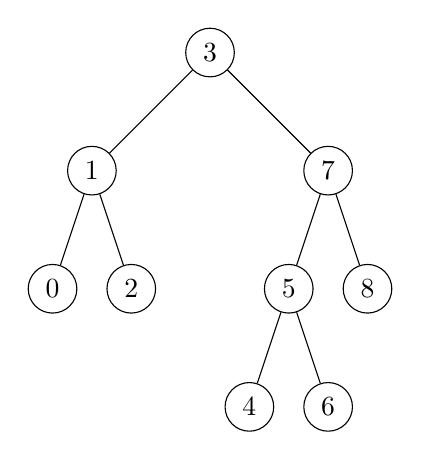
\begin{tikzpicture}
      [level 1/.style={sibling distance=30mm},
       level 2/.style={sibling distance=15mm},
       level 2/.style={sibling distance=10mm}]
      \tikzstyle{every node}=[circle,draw]
      \node{3}
      child{
        node{1}
        child{node{0}}
        child{node{2}}
      }
      child{
        node{7}
        child{
          node{5}
          child{node{4}}
          child{node{6}}
        }
        child{node{8}}
      };
    \end{tikzpicture} \hspace{4mm}
    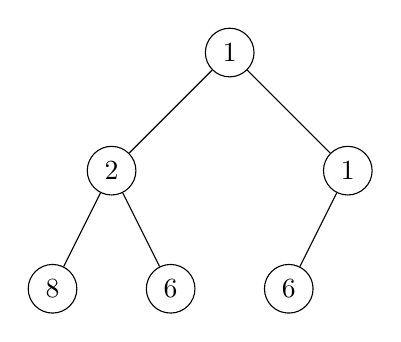
\begin{tikzpicture}
      [level 1/.style={sibling distance=30mm},
       level 2/.style={sibling distance=15mm}]
      \tikzstyle{every node}=[circle,draw]
      \node{1}
      child{
        node{2}
        child{node{8}}
        child{node{6}}
      }
      child{
        node{1}
        child{node{6}}
        child[missing]{node{k}}
      }
      ;
    \end{tikzpicture} \hspace{4mm}
    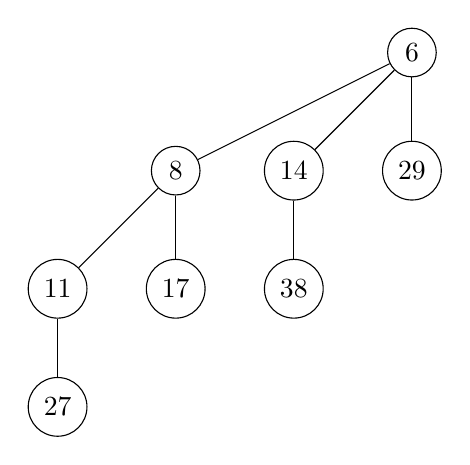
\begin{tikzpicture}[grow via three points={%
        one child at (0,-1.5) and two children at (0,-1.5) and (-1.5,-1.5)}]
      \tikzstyle{every node}=[circle,draw]
      \node at (0,0) {6}
      child{node{29}}
      child{
        node{14}
        child{
          node{38}
        }
      }
      child{
        node{8}
        child{node{17}}
        child{
          node{11}
          child{node{27}}
        }
      }
      ;
    \end{tikzpicture}
  \end{center}
  \caption{A binary search tree (on the left), a binary min-heap (in
    the middle), and a binomial tree of rank $3$ (on the right).}
  \label{fig:trees}
\end{figure}

Algorithms can be typeset as pseudo-code as exemplified in
Algorithm~\ref{algo:demo}: study its \LaTeX\ source code.

\begin{algorithm}[t]
  \begin{algorithmic}[1]  % comment [1] away to drop the line numbers
    \STATE \Function $f(n)$
    \IF[optional comment]{$n < 0$}
      \STATE $n \IsAssigned -2 \cdot n$ \COMMENT{optional comment}
    \ELSE[$n \geq 0$]
      \STATE $n \IsAssigned  3 \cdot n$
    \ENDIF
    \WHILE[optional comment]{$n > 0$}
      \STATE $n \IsAssigned n-1$
    \ENDWHILE
    \RETURN $n$
  \end{algorithmic}
  \caption{Silly algorithm}
  \label{algo:demo}
\end{algorithm}

If you are not sure whether you will stick to your current choice of
notation or terminology, then introduce a new (possibly parametric)
command.  For example, upon
\begin{center}
  \verb|\newcommand{\Cardinality}[1]{\left\lvert#1\right\rvert}|
\end{center}
the formula \verb|$\Cardinality{S}$| typesets the cardinality of set
$S$ as $\Cardinality{S}$ with autosized vertical bars and proper
spacing, but upon changing the definition of that parametric command
to
\begin{center}
  \verb|\newcommand{\Cardinality}[1]{\# #1}|
\end{center}
and recompiling, the formula \verb|$\Cardinality{S}$| typesets the
cardinality of set $S$ as $\#S$.
%
Similarly, upon
\begin{center}
  \verb|\newcommand{\MiniZinc}{\textit{Mini\-Zinc}}|
\end{center}
the text \verb|\MiniZinc\| typesets into \textit{MiniZinc},
hyphenation being only possible in the middle, but upon changing the
definition of that non-parametric command to
\begin{center}
  \verb|\newcommand{\MiniZinc}{\textsc{Mini\-Zinc}}|
\end{center}
and recompiling, the text \verb|\MiniZinc\| typesets into
\textsc{MiniZinc}.
%
You can thus obtain an arbitrary number of changes in the document
with a \emph{constant}-time change in its source code, rather than
having to perform a \emph{linear}-time find-and-replace operation
within the source code, which is painstaking and error-prone.  The
imported file \texttt{macros.tex} has a lot of useful predefined
commands about mathematics, CP, \Gecode, modelling, \MiniZinc, and
algorithms.

Use commands on positioning (such as \verb|\hspace|, \verb|\vspace|,
and \verb|\noindent|) and appearance (such as \verb|\small| for
reducing the font size, and \verb|\textit| for italics) very
sparingly, and ideally only in (parametric) commands, as the very idea
of mark-up languages such as \LaTeX\ is to let the class designer
(usually a trained professional typesetter) decide on where things
appear and how they look.  For example, \verb|\emph| (for emphasis)
compiles (outside italicised environments, such as \texttt{theorem})
into \textit{italics} under the \texttt{article} class used for this
document, but it may compile into \textbf{boldface} under some other
class.
\begin{center}
  \textbf{If you do not (need to) worry about \emph{how} things look, \\
    then you can fully focus on \emph{what} you are trying to
    express!}
\end{center}

Note that \emph{no} absolute numbers are used in the \LaTeX\ source
code for any of the references inside this document.  For ease of
maintenance, \verb|\label| is used for giving a label to something
that is automatically numbered (such as an algorithm, equation,
figure, footnote, item, line, part, section, subsection, or table),
and \verb|\ref| is used for referring to a label.  An item in the
bibliography file is referred to by \verb|\cite| instead.  Upon
changing the text, it suffices to recompile, once or twice, and
possibly to run BibTeX again, in order to update all references
consistently.

Always write
%
\verb| Table|$\sim$\verb|\ref{tab:maths} |
%
instead of
%
\verb| Table \ref{tab:maths}|,
%
by using the non-breaking space (which is typeset as the tilde $\sim$)
instead of the normal space, because this avoids that a
cross-reference is spread across a line break, as for example in
``Table \ref{tab:maths}'', which is considered poor typesetting.

The rules of English for how many spaces to use before and after
various symbols are given in Table~\ref{tab:spacing}.  Beware that
they may be very different from the rules in your native language.

\begin{table}[h]
  \centering
  \begin{tabular}{|c|c|c|c|}
    \cline{3-4}
    \multicolumn{2}{c|}{} & \multicolumn{2}{c|}{number of spaces after} \\
    \cline{3-4}
    \multicolumn{2}{c|}{} & 0 & 1 \\
    \hline
    \multirow{2}{*}{number of spaces before} & 0 & / - & , : ; . ! ?
    ) ] \} ' '' \% \\
    \cline{2-4}
    & 1 & ( [ \{ ` `` & -- (\emph{n}-dash) --- (\emph{m}-dash) \\
    \hline
  \end{tabular}
  \caption{Spacing rules of English}
  \label{tab:spacing}
\end{table}

\vfill

\noindent
\handpoint\ Feel free to report to the instructor any other features
that you would have liked to see discussed and exemplified in this
template document.


\end{document}

%%% Local Variables:
%%% mode: latex
%%% TeX-master: t
%%% End:
